
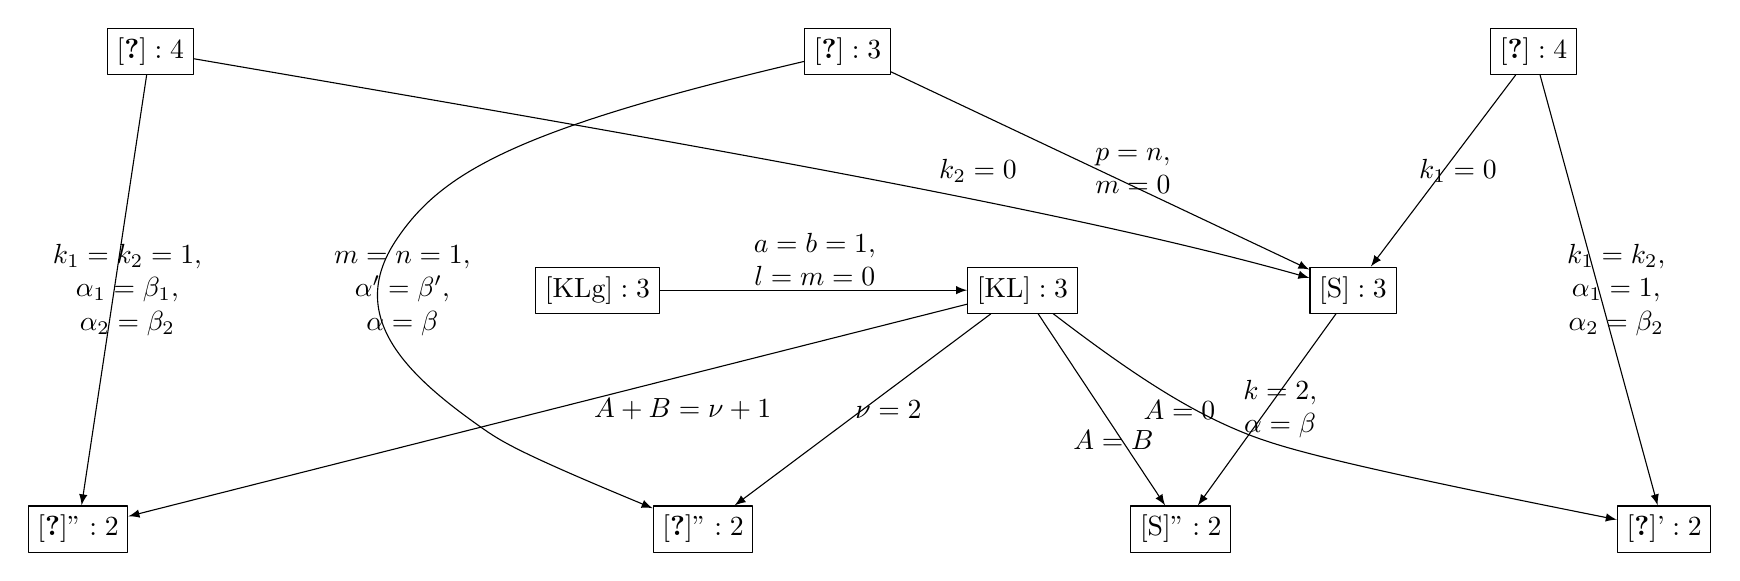
\begin{tikzpicture}[>=latex,line join=bevel,]
%%
\begin{scope}
  \pgfsetstrokecolor{black}
  \definecolor{strokecol}{rgb}{1.0,1.0,1.0};
  \pgfsetstrokecolor{strokecol}
  \definecolor{fillcol}{rgb}{1.0,1.0,1.0};
  \pgfsetfillcolor{fillcol}
\end{scope}
\begin{scope}
  \pgfsetstrokecolor{black}
  \definecolor{strokecol}{rgb}{1.0,1.0,1.0};
  \pgfsetstrokecolor{strokecol}
  \definecolor{fillcol}{rgb}{1.0,1.0,1.0};
  \pgfsetfillcolor{fillcol}
\end{scope}
\begin{scope}
  \pgfsetstrokecolor{black}
  \definecolor{strokecol}{rgb}{1.0,1.0,1.0};
  \pgfsetstrokecolor{strokecol}
  \definecolor{fillcol}{rgb}{1.0,1.0,1.0};
  \pgfsetfillcolor{fillcol}
\end{scope}
  \node (KLg) at (287.16bp,104.0bp) [draw,rectangle] {${\mbox{[KLg]}}:3$};
  \node (Spp) at (497.16bp,18.0bp) [draw,rectangle] {$\mbox{[S]''}:2$};
  \node (KL) at (440.16bp,104.0bp) [draw,rectangle] {${\mbox{[KL]}}:3$};
  \node (S) at (559.16bp,104.0bp) [draw,rectangle] {$\mbox{[S]}:3$};
  \node (DF85) at (377.16bp,190.0bp) [draw,rectangle] {$\mbox{\cite{dotsenko1985four}}:3$};
  \node (War10) at (126.16bp,190.0bp) [draw,rectangle] {$\mbox{\cite{warnaar2010sl3}}:4$};
  \node (War10pp) at (100.16bp,18.0bp) [draw,rectangle] {$\mbox{\cite{warnaar2010sl3}''}:2$};
  \node (DF85pp) at (325.16bp,18.0bp) [draw,rectangle] {$\mbox{\cite{dotsenko1985four}''}:2$};
  \node (TV03) at (624.16bp,190.0bp) [draw,rectangle] {$\mbox{\cite{tarasov2003selberg}}:4$};
  \node (TV03p) at (671.16bp,18.0bp) [draw,rectangle] {$\mbox{\cite{tarasov2003selberg}'}:2$};
  \draw [->] (KLg) ..controls (355.95bp,104.0bp) and (364.52bp,104.0bp)  .. (KL);
  \definecolor{strokecol}{rgb}{0.0,0.0,0.0};
  \pgfsetstrokecolor{strokecol}
  \draw (365.41bp,114.0bp) node {$\begin{array}[]{c}a=b=1,\\l=m=0\end{array}$};
  \draw [->] (DF85) ..controls (257.57bp,161.95bp) and (230.84bp,146.31bp)  .. (214.66bp,122.0bp) .. controls (196.21bp,94.272bp) and (218.87bp,73.092bp)  .. (246.16bp,54.0bp) .. controls (253.17bp,49.094bp) and (260.96bp,44.594bp)  .. (DF85pp);
  \draw (216.91bp,104.0bp) node {$\begin{array}[]{c}m=n=1,\\ \alpha'=\beta',\\\alpha=\beta\end{array}$};
  \draw [->] (TV03) ..controls (601.33bp,159.79bp) and (589.34bp,143.93bp)  .. (S);
  \draw (596.91bp,147.0bp) node {$k_1=0$};
  \draw [->] (KL) ..controls (399.03bp,73.243bp) and (376.04bp,56.048bp)  .. (DF85pp);
  \draw (391.91bp,61.0bp) node {$\nu=2$};
  \draw [->] (TV03) ..controls (637.32bp,141.85bp) and (653.84bp,81.379bp)  .. (TV03p);
  \draw (653.91bp,104.0bp) node {$\begin{array}[]{c}k_1=k_2,\\ \alpha_1=1,\\\alpha_2=\beta_2\end{array}$};
  \draw [->] (KL) ..controls (477.67bp,75.267bp) and (497.4bp,62.231bp)  .. (516.66bp,54.0bp) .. controls (530.58bp,48.051bp) and (545.64bp,42.997bp)  .. (TV03p);
  \draw (517.91bp,61.0bp) node {$\kern-1.5cm A=0$};
  \draw [->] (War10) ..controls (118.9bp,141.98bp) and (109.82bp,81.897bp)  .. (War10pp);
  \draw (117.91bp,104.0bp) node {$\begin{array}[]{c}k_1=k_2=1,\\\alpha_1=\beta_1,\\\alpha_2=\beta_2\end{array}$};
  \draw [->] (DF85) ..controls (443.47bp,158.67bp) and (481.94bp,140.49bp)  .. (S);
  \draw (479.91bp,147.0bp) node {$\begin{array}[]{c}p=n,\\m=0\end{array}$};
  \draw [->] (KL) ..controls (460.19bp,73.79bp) and (470.7bp,57.933bp)  .. (Spp);
  \draw (472.91bp,61.0bp) node {$\begin{array}[]{c}\\\\A=B\end{array}$};
  \draw [->] (S) ..controls (537.38bp,73.79bp) and (525.95bp,57.933bp)  .. (Spp);
  \draw (532.91bp,61.0bp) node {$\begin{array}[]{c}k=2,\\\alpha=\beta\end{array}$};
  \draw [->] (War10) ..controls (319.57bp,156.83bp) and (456.39bp,132.93bp)  .. (S);
  \draw (424.11bp,147.0bp) node {$k_2=0$};
  \draw [->] (KL) ..controls (327.99bp,75.626bp) and (243.53bp,54.264bp)  .. (War10pp);
  \draw (292.91bp,61.0bp) node {$\kern5emA+B=\nu+1$};
%
\end{tikzpicture}
